\documentclass[12pt]{article}
\usepackage{mathtools}
\usepackage[shortlabels]{enumitem}
% make sure to keep these two lines the very last in the preamble
% if you want to add packages add them before not after these two lines
\usepackage[subpreambles=true]{standalone}

\begin{document}
\section{Tests et Resultats}
Dans cette partie, nous allons comparer les performances de nos algorithmes implémentés, pour cela, en premier lieu on va utiliser notre propre générateur d’instances pour comparer les 4 algorithms : recherche exhaustive , Branch \& Bound , Branch \& Bound amélioré. ensuite on utilisera les instances du benchmark Scholl. 
\paragraph*{Remarque: } Les algorithmes ont été développés en utilisant le langage de programmation Python, et exécutés sur un \textbf{HP probook [Intel Core i7-6500U CPU @2.50GHz, 8Go RAM ]} en utilisant l'IDE Intellij pycharm
Le générateur d’instances utilise la fonction random() de la bibliothèque random de Python, cette fonction utilise le Mersenne Twister qui est un générateur de nombres pseudo-aléatoires, réputé pour sa qualité.
\subsection{Instances générées : }
On génère plusieurs instances du problèmes avec la valeur \(C=100\) pour la capacité de la boîte, et un nombre d’articles croissant : \( N \in \{5,10,15,20,25\}\). Les volumes des articles sont générés aléatoirement dans l’interval \(]0,100]\). le tableau ci dessous résume les résultats en termes de temps d'exécution en secondes de chacun des 4 algorithmes sur les instances générées. 
\begin{figure}[H]
    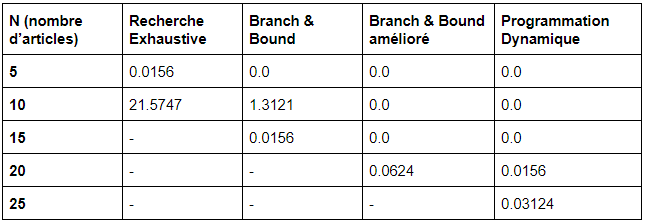
\includegraphics[width=13.5cm]{../figures/tab1.png}
\end{figure}
\begin{figure}[H]
    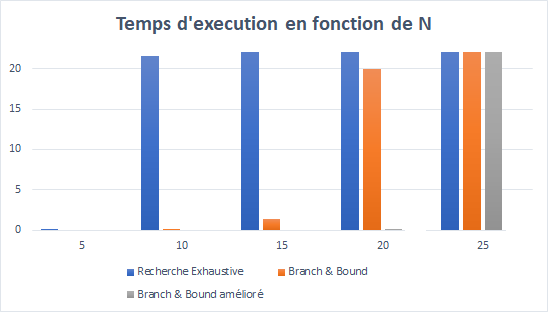
\includegraphics[width=13.5cm]{../figures/graph1.png}
\end{figure}
\subsubsection{Analyse des résultats:}
\begin{enumerate}
    \item On remarque d’un côté qu’en augmentant la taille du problème, le temps d'exécution augmente très rapidement.
    \item D’un autre côté, les performances de la DP sont meilleures que celle du Branch and Bound amélioré , suivie du Branch \& Bound classique, et enfin vient la rechercher exhaustive qui prend un temps énorme pour résoudre des instances de taille petite. 
    \item Le Branch \& Bound et la recherche exhaustive arrivent rapidement à leur limite ,qui est de \(N=15\) et \(N=20\) respectivement, suivi du Branch and Bound pour \(N=25\) dans ces instances générées. Ceci signifie que ces méthodes ne sont pas efficaces pour de grandes instances.
\end{enumerate}
\subsubsection{Interprétation des résultats:}
On justifie les résultats obtenus et la grande différence entre les temps d’exécution des 4 méthodes comme suit: 
\begin{enumerate}
    \item La recherche exhaustive, donne des temps d'exécution les plus long, car cette dernière ne possède aucun mécanisme de réduction du problème, donc elle vas parcourir toute les permutations possibles des articles.
    \item Le Branch \& Bound, offre une petite amélioration par rapport à la recherche exhaustive, grâce à la borne inférieure L1 utilisée pour réduire quelques branches qu’on est sure qu’elles ne contiennent pas la solution optimale, mais cet algorithme arrive à sa limite rapidement, car la borne L1 n’est efficace que lorsque les volume des articles sont petits par rapport à la capacité de la boîte, sinon, on retombe sur une recherche exhaustive.
    \item Le Branch \& Bound amélioré, augmente les performances du Branch \& Bound classique, à cause de la borne L2 qui couvre des cas de réduction plus large que la borne L1, de plus , l’utilisation des heuristiques permet d'accélérer le temps de trouver un noeud exacte.
\end{enumerate}
\subsection{Scholl Benchmark:}
le Scholl benchmark est composé de 3 différentes classes, les volume des articles sont uniformément distribués entre 50 et 500. la capacité C de la boîte est entre 100 et 150 dans la première classe (Scholl1), égale à 1000 dans la classe 2 ( Scholl2) et égale à 100 000 dans la 3ème classe (Scholl3). 
les deux algorithmes Recherche exhaustive et Branch \& Bound sont incapable de résoudre les instances de ce benchmark à cause de leurs tailles et difficulté relativement élevés. Donc, dans cette partie nous étudier Branch \& Bound amélioré [BBA]. 

Pour chaque classe, on a 4 valeurs de N (50,100,200,500) et pour chaque couple (N,C) on prends 5 instances afin de calculer le temps d'exécution moyen, ceci est dû à la génération aléatoire des volume des articles, ce qui peut rendre quelques instances plus difficiles que d’autres, même s’ils ont la même valeur du couple (N,C) . les résultats en temps d'exécution sont présentés dans le tableau suivant:
\begin{figure}[H]
    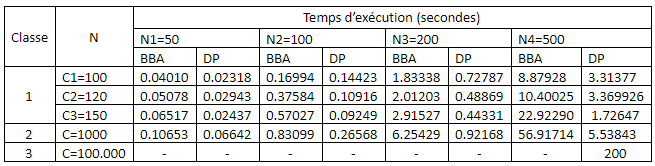
\includegraphics[width=13.5cm]{../figures/tab2.png}
\end{figure}
\subsubsection{Analyse des résultats:}
\begin{enumerate}
    \item En augmentant N le nombre d’articles, le temps d'exécution augmente d’une façon exponentielle
    \begin{figure}[H]
        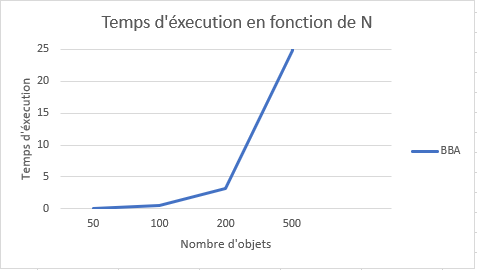
\includegraphics[width=13.5cm]{../figures/BBA_TEXEC_N.PNG}
    \end{figure}
    \item En fixant le nombre d’articles, l’augmentation de la capacité C produit une augmentation dans les temps d’exécution
    \begin{figure}[H]
        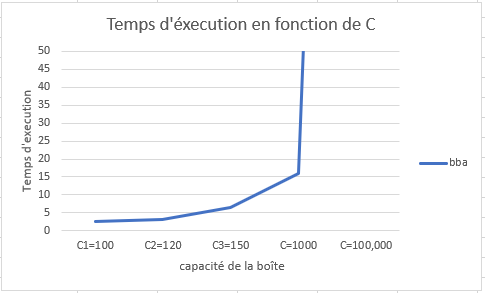
\includegraphics[width=13.5cm]{../figures/BBA_TEXEC_C.PNG}
    \end{figure}
    \item Pour la 3eme classe, qui contient les instances les plus difficiles, seul l’algorithme DP arrive à terminer son exécution( en 200 secondes), ce qui n’est pas très intéressant comme temps d'exécution.
\end{enumerate}
\subsubsection{Conclusion méthodes exactes}
Malgré les améliorations apportées aux algorithmes exactes ( utilisation des heuristiques pour l’initialisation de la solution optimale, utilisation d’un évaluation plus performante ..), ces derniers suivent toujours la courbe exponentielle en terme de temps d'exécution en augmentant la taille du problème. En d’autres termes, ce type d’algorithmes arrivent rapidement à leur limite, sans même pas pouvoir résoudre des instances de taille moyenne.
De nos jours, les données étants d’une très grande taille ( qui dépasse les milliers ), l’utilisation des méthodes exactes, quelques soit leurs performances, est impossible même avec les ordinateurs les plus rapides du monde. C’est pour cela que les chercheurs se sont dirigés vers des méthodes approchées qui fournissent une solution proche de l’optimal mais en un temps polynomial. Ce qui fait l’article des prochaines parties de notre projet.

\end{document}